
\chapter{Ejemplo práctico: Text Mining con R}
\label{cha:Text-mining-r}

En este capítulo se va a desarrollar un caso práctico sobre minería de textos, con el fin de corroborar 
su utilidad y su importancia en el mundo actual. Para dicho análisis necesitaremos una fuente de 
información de donde extraer los textos a analizar, dicha fuente bien podría ser un artículo de opinión, 
discursos transcritos…El conjunto de textos a analizar, serán publicaciones de los últimos tres presidentes 
de Estados Unidos, en este caso en Twitter, con el fin de analizar dichas publicaciones y realizar un estudio
sobre las mismas.

Twitter es actualmente una dinámica e ingente fuente de contenidos que, dada su popularidad e impacto, 
se ha convertido en la principal fuente de información para estudios de Social Media Analytics. Multitud 
de empresas emplean este tipo de técnica para obtener información muy valiosa de individuos o de 
corporaciones. Análisis de reputación de empresas, productos o personalidades, estudios de impacto 
relacionados con marketing, extracción de opiniones y predicción de tendencias son sólo algunos ejemplos 
de aplicaciones.

Además de R existen otros lenguajes de programación como Python, MatLab u Octave. Si bien Python es el 
lenguaje que domina en este ámbito, este análisis se realizará a través de la programación en R, pues 
contiene tanto librerías, como paquetes que facilitan y extienden sus capacidades como herramienta de 
análisis de texto.


\section{Introducción}
\label{sec:introduccion}

Tal y como ocurre en muchas redes sociales, Twitter otorga la posibilidad de compartir sus datos tanto 
con empresas como con desarrolladores y/o usuarios particulares. Aunque en la mayoría de casos se trata 
de web Services API, con frecuencia existen librerías que permiten interactuar con la API desde diversos 
lenguajes de programación. 

La forma en la que Twitter permite acceder a su contenido es a través de lo que se conoce como Twitter 
App, al crear dicha Twitter App, se adquieren una serie de claves y tokens de identificación que 
permiten acceder a la aplicación y consultar la información necesaria.  

Algo que se deberá tener en cuenta durante este análisis, es que Twitter tiene una normativa que regula 
la frecuencia máxima de peticiones, así como la cantidad máxima de tweets que se pueden extraer. Durante 
la fase de extracción de la información, se deberá tener en cuenta dichos limites con el objetivo de 
evitar ser sancionado por la organización.

\section{Acceso a la API}
\label{sec:acceso-api}

Para acceder a la API de Twitter, como se indica en la documentación de la misma, existen dos métodos de 
acceso Oauth2 y Oauth1a. El acceso con cada uno de ellos dependerá del tipo de información que se desee 
extraer \cite{oauth1a}. Como veremos a continuación, el metodo de acceso elegido será Oauth1a.

\begin{figure}[tphb]
  		   \centering
     		   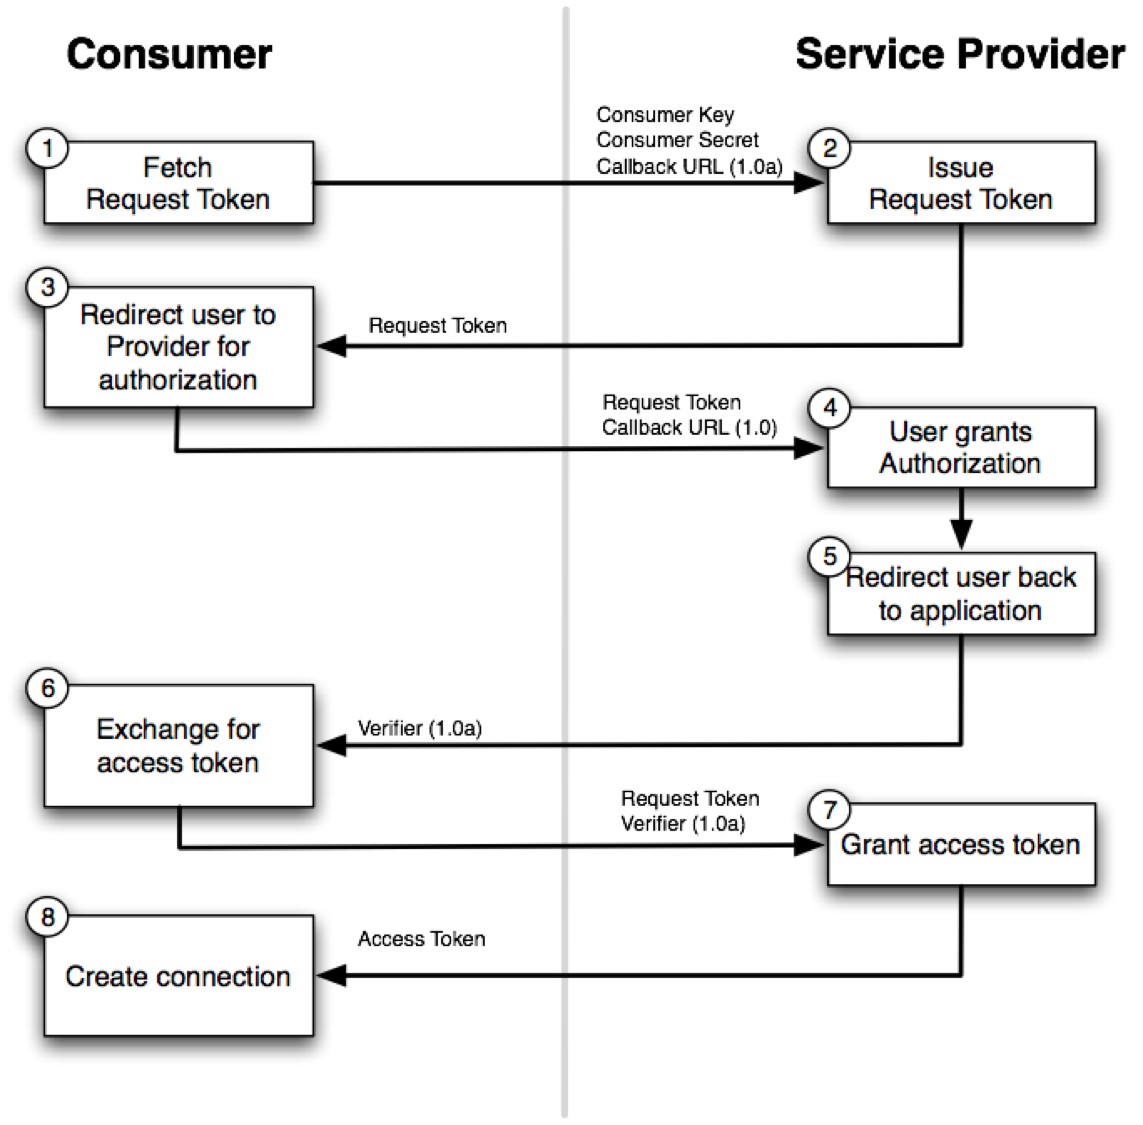
\includegraphics[width=4.5in]{Oauth1a.png}
  		   \caption{Funcionamiento de Oauth1a}
  		   \label{img:oauth1a}
\end{figure}

Puesto que se desea extraer información específica de algunos usuarios de la plataforma, el metodo de 
acceso será a través de Oauth1a. Así pues, OAuth1a para funcionar requiere 
de cuatro elementos que provienen de la aplicación de Twitter creada por el usuario desarrollador, estos elementos son:

\begin{enumerate}
	\item Clave del consumidor
	\item Clave del consumidor secreta
	\item Token de acceso
	\item Token de acceso secreto
\end{enumerate}


Todos estos recursos deberán ser proporcionados por la plataforma de Twitter para desarrolladores. Una 
vez se disponen de dichos recursos, realizamos el proceso de identificación y obtención de tokens \cite{error_oauth1a}, 
no sin antes cargar las librerías necesarias para el desarrollo de dicho caso práctico.


\begin{Schunk}
\begin{Sinput}
>   #En primer lugar se cargan las librerias necesarias.
>   library(twitteR)
>   library(tidyverse)
>   library(knitr)
\end{Sinput}
\end{Schunk}






Una vez que las librerías necesarias están cargadas, se procede a crear las variables que almacenarán los 
recursos de acceso. A conitnuación, se llama a la función de acceso, proporcionando los parametros anteriormente definidos.
Esta función envuelve las funciones de protocolo de enlace de autenticación OAuth 1.0 del paquete httr para una sesión de Twitter 
en concreto. \cite{create_token}.


\begin{Schunk}
\begin{Sinput}
>   #Ahora se definen ciertas variables que almacenaran la informacion de acceso
>   nombre_app <- "MarquezDavidTFG"
>   clave <- "bsS2cbbZe7BDsxFPLYRM0GKJ8"
>   clave_secreta <- "WvUilwEZbgJhHiUgpjyboQcQHYSSCNKwImHF1TeINe9aWskkDo"
>   token_acceso <- "3147132436-kFG9XkuWsdI8n1KPVZQTOrf6rw45lrqPEPoUXPr"
>   token_acceso_secreto <- "zK8dyBAgB4sTrRhjVBXmNCAjX4QQvCUfQIXckQmTrcAix"

>   #Acceso a la API
>   options(httr_oauth_cache=TRUE)
>   setup_twitter_oauth(consumer_key = clave, consumer_secret = clave_secreta, access_token = token_acceso, access_secret = token_acceso_secreto)
\end{Sinput}
\end{Schunk}


\section{Extracción y carga de datos}
\label{sec:extraccion-carga-datos}

Una vez que se ha conseguido acceder a la API a través de la aplicación para desarrolladores proporcionada por Twitter, se procede 
con la fase de extracción de datos. Como se ha indicado en la sección \ref{sec:introduccion}, en Twitter existe una normativa 
que regula la frecuencia máxima de peticiones, así como la cantidad máxima de tweets que se pueden extraer \cite{rate_limit}. Para 
el tipo de análisis que se quiere realizar en este trabajo, se pretenden obtener la mayor cantidad de tweets posible, puesto que el 
número máximo de publicaciones que se pueden extraer por consulta son 200, se sigue la siguiente estrategia:

\begin{enumerate}
	\item Toda publicación  tiene un identificador numérico global, que sigue un orden temporal. Esto permitirá identificar y distinguir 
	los tweets mas recientes de los más antiguos.

	\item Es posible recuperar y trabajar solo con publicaciones antiguas, empelando como parámetro de la función el identificador de 
	cada tweet.

	\item Antes de cada consulta, se lee el fichero donde se almacenan las publicaciones y se identifica el ID del ultimo tweets
	recuperado. Si no existe dicho fichero de almacenamiento para el usuario en cuestión, se crea uno.

	\item Se realiza una nueva consulta empleando como argumento maxID el identificador recuperado en el paso anterior.

	\item Se incorporan los nuevos datos al archivo de almacenamiento.
\end{enumerate} 

Una vez ha quedado claro el proceso de extracción, se pasa a crear una función que se encargue de dicha tarea \footnote{Se puede consultar 
más información sobre la implementación de dicha función en el apéndice \ref{sec:funcion-extraccion}, donde se detalla el funcionamiento y uso 
de la misma.}. Cada vez que se ejecute dicha función, se recuperan nuevo tweets y se almacenan junto a los ya extraídos previamente.


\begin{Schunk}
\begin{Sinput}
>   extraccion_tweets(usuario  = "JoeBiden", maxtweets  = 200)
>   extraccion_tweets(usuario  = "DonaldTrump", maxtweets  = 200)
>   extraccion_tweets(usuario  = "BarackObama", maxtweets  = 200)
\end{Sinput}
\end{Schunk}






